\chapter{Linguaggi Regolari o Lineari}

%%%%%%%%%%%%%%%%%%%%%%%%%%%%%%%%%%%%%%%%%%%%%%%%%%%%%%%%%%%%%%%%%%%%%%%%%%%%%%%%%%%%%%%%%%%%%%%%%%%%%%%%%%%%%%%%%%%
\section{Da DFA a Grammatica Regolare}

Una grammatica \'e regolare se le produzioni sono della forma: $A \rightarrow \beta$, con $\beta$ terminale non-terminale, viceversa o 
terminale e basta.\\[5pt]

\begin{center}
    \begin{tabular}{lll}
        $A \rightarrow aB$     &    $B \rightarrow b$   &   grammatica lineare destra\\
        $B \rightarrow Ab$     &    $A \rightarrow a$   &   grammatica lineare sinistra\\
    \end{tabular}
\end{center}

Dato un DFA D voglio trovare una grammatica regolare G tale che L(G) = L(D). 
Se ho una transizione $A \rightarrow B$ con una a-transizione diventer\'a $A \rightarrow aB$. Segno il nome del nodo che sto considerando
prima della freccia e, dopo la freccia, il non terminale ed il nodo destinazione. Se ho un nodo foglia C avr\'o  $C \rightarrow \varepsilon$.

Se invece ho una grammatica regolare e voglio trovare un DFA D $/\ L(G) = L(D)$, faccio il procedimento inverso a prima;
se ottengo un NFA basta fare Subset Construction.

%%%%%%%%%%%%%%%%%%%%%%%%%%%%%%%%%%%%%%%%%%%%%%%%%%%%%%%%%%%%%%%%%%%%%%%%%%%%%%%%%%%%%%%%%%%%%%%%%%%%%%%%%%%%%%%%%%%5
\subsection{Esempio}
$L=\{ w \ / \ w \in \{ a, b \} ^* \&\& |a|\ pari,\ |b|\ dispari \}$, L \'e regolare?
\begin{center}
	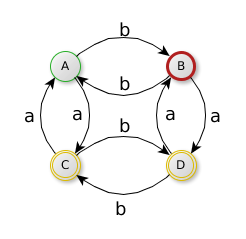
\includegraphics[scale=0.5]{Chapters/Img/c02_12.png}\\
\end{center} 
S\'i \'e regolare.

%%%%%%%%%%%%%%%%%%%%%%%%%%%%%%%%%%%%%%%%%%%%%%%%%%%%%%%%%%%%%%%%%%%%%%%%%%%%%%%%%%%%%%%%%%%%%%%%%%%%%%%%%%%%%%%%%%%5
\subsection{Considerazioni}
\begin{tcolorbox}\begin{center}
    Regular expression, NFA e DFA hanno la stessa potenza espressiva, sono solo notazioni diverse.\\
\end{center}\end{tcolorbox}

\begin{tcolorbox}\begin{center}
    Dal DFA posso sempre costruirmi una \textbf{grammatica regolare} equivalente.\\
\end{center}\end{tcolorbox}

\begin{tcolorbox}\begin{center}
    Non devo fare l'errore di assumere che qualsiasi grammatica sia esprimibile attraverso un NFA.\\
\end{center}\end{tcolorbox}
%%%%%%%%%%%%%%%%%%%%%%%%%%%%%%%%%%%%%%%%%%%%%%%%%%%%%%%%%%%%%%%%%%%%%%%%%%%%%%%%%%%%%%%%%%%%%%%%%%%%%%%%%%%%%%%%%%%5
\subsection{Esempio}
$L=\{ w \ / \ w \in \{ a, b \} ^* \&\& |a|=|b|\}$, L \'e regolare?
\begin{center}
	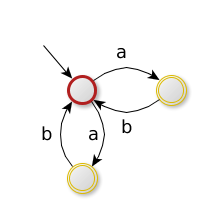
\includegraphics[scale=0.5]{Chapters/Img/c02_13.png}\\
\end{center} 
Non potr\'a mai essere regolare, per il pumping lemma per i linguaggi regolari.

%%%%%%%%%%%%%%%%%%%%%%%%%%%%%%%%%%%%%%%%%%%%%%%%%%%%%%%%%%%%%%%%%%%%%%%%%%%%%%%%%%%%%%%%%%%%%%%
\section{Pumping Lemma per Linguaggi Regolari}

Sia L un linguaggio regolare
$\implies \exists\ p \in \mathbb{N}^+ \ / \ \forall\ z \in L \ / \ |z| > p$,
$\exists\ u,v,w \ / \ $:

\begin{itemize}
    \item[i)] $z = uvw\ \land$\\
    \item[i)] $|uw| \leq p\ \land$\\
    \item[i)] $|v| > 0,\ \forall i \in \mathbb{N},\ u v^i w \in L$\\
\end{itemize}

%%%%%%%%%%%%%%%%%%%%%%%%%%%%%%%%%%%%%%%%%%%%%%%%%%%%%%%%%%%%%%%%%%%%%%%%%%%%%%%%%%%%%%%%%%%%%%%
\subsection{Dimostrazione}
L \'e regolare quindi pu\'o essere riconosciuto da un automa a stati finiti.\\
Sia D il min DFA $\ / \ L(D) = L,\ p = |S|$, allora i cammini pi\'u lunghi che non passano pi\'u di una volta nel medesimo 
stato hanno al pi\'u lunghezza (p-1).\\
Allora se $z \in L$ con $|z|>p$, z \'e riconosciuta tramite un cammino che attraversa almeno due volte uno stato. \\

%%%%%%%%%%%%%%%%%%%%%%%%%%%%%%%%%%%%%%%%%%%%%%%%%%%%%%%%%%%%%%%%%%%%%%%%%%%%%%%%%%%%%%%%%%%%%%%%%%%%%%%%%%%%%%%%%%%5
\subsection{Negazione testi Pumping Lemma per linguaggi regolari}
$\forall p \in \mathbb{N}^+ \ / \ \exists\ z \in L \ / \ |z| > p.\ \forall\ uvw $
$z = uvw \land |uw| \leq p \land |v| > 0) \implies \exists\ i \in \mathbb{N} \ / \ u v^i w \not\in L) $

Lemma: $L=\{a^nb^n \ / \ n \geq 0\}$ non \'e regolare\\
Dim: Assumo per assurdo che L sia regolare, dato p un qualunque numero positivo e $z= a^p b^p $ allora
$\forall\ uvw \ / \ z = uvw \land |uw| \leq p \land |v| > 0$ (la stringa v contiene solo (e almeno una) \lq a\rq ).

allora $uv^2w$ ha la forma $a^{p+k}b^p,\ k > 0$
allora $uv^2w \not\in L$ il che contraddice il Pumping Lemma per linguaggi regolari.

%%%%%%%%%%%%%%%%%%%%%%%%%%%%%%%%%%%%%%%%%%%%%%%%%%%%%%%%%%%%%%%%%%%%%%%%%%%%%%%%%%%%%%%%%%%%%%%%%%%%%%%%%%%%%%%%%%%5
\subsection{Esercizio}
$L_1 = \{ w \ / \ w \in \{ a, b \}^* \text{e contiene almeno una occorrenza di \lq\lq aa \rq\rq}\}$\\

$L_1$:
$A \rightarrow aA | bA | aB$\\
$B \rightarrow aC$\\
$C \rightarrow aC | bC | \varepsilon $\\

$L_2 = \{ ww \ / \ \ \in \{ a,b \}^* \}$\\
non \'e libero per il pumping lemma (gi\'a dimostrato), quindi non \'e regolare.

$L_3 = \{ww^r \ / \ w \in \{ a,b \}^* \}$\\
Non \'e regolare ma libero.
$z = a^p b^p b^p a^p \in L_3$
visto che $uv < p$, uv \'e composta solo da a 
$u v^i w = a^pb^{2p}a^p \not\in L_3$ quindi non pu\'o essere regolare.

%%%%%%%%%%%%%%%%%%%%%%%%%%%%%%%%%%%%%%%%%%%%%%%%%%%%%%%%%%%%%%%%%%%%%%%%%%%%%%%%%%%%%%%%%%%%%%%%%%%%%%%%%%%%%%%%%%%5
\subsection{Esercizi di esame}
Sia $N_1$ lo NFA con stato iniziale A e finale E con la seguente funzione di transizione:

\begin{center}
    \begin{tabular}{|c|c|c|c|}
        \hline
            &   $\varepsilon$      &   a           &   b           \\
        \hline
            A    &   $\{B, E\}$ &   $\o$        &  $\o$         \\
        \hline
            B    &   $\{ C \}$  &   $\o$        &  $\{ E \}$    \\
        \hline
            C    &   $\o$       &   $\{ D \}$   &  $\o$         \\
        \hline
            D    &   $\{ E \}$  &   $\o$        &  $\{ B \}$    \\
        \hline
            E    &   $\o$       &    $\{ E \}$  &  $\{ A \}$    \\
        \hline
    \end{tabular}
\end{center} 

\begin{itemize}
    \item[1)] $aa \in L(N_1)$?\\
    \item[2)] D \'e il DFA ottenuto da $N_1$, per subset construction, Q stato iniziale di D, $Q_{ab\_}$ lo stato di D che si 
    raggiunge da Q tramite il cammino ab. Dire a quale sottoinsieme degli stati di $N_1$ corrisponde $Q_{ab\_}$.\\    
\end{itemize}

1) S\'i facendo $A \rightarrow B \rightarrow C \rightarrow D \rightarrow E \rightarrow E $
2) Facendo la subset construction:

\begin{center}
    \begin{tabular}{|l|l|l|}
        \hline
                                &   a   &  b    \\
        \hline
            $Q0 = \{A,B,C,D\}$  &   Q1  &  Q0   \\
        \hline
            $Q1 = \{D,E\}$      &   Q2  &  Q0   \\
        \hline
           $Q2 = \{E\}$         &   Q2  &  Q0   \\
        \hline
    \end{tabular}
\end{center} 